\documentclass{article}\usepackage[]{graphicx}\usepackage[]{color}
%% maxwidth is the original width if it is less than linewidth
%% otherwise use linewidth (to make sure the graphics do not exceed the margin)
\makeatletter
\def\maxwidth{ %
  \ifdim\Gin@nat@width>\linewidth
    \linewidth
  \else
    \Gin@nat@width
  \fi
}
\makeatother

\definecolor{fgcolor}{rgb}{0.345, 0.345, 0.345}
\newcommand{\hlnum}[1]{\textcolor[rgb]{0.686,0.059,0.569}{#1}}%
\newcommand{\hlstr}[1]{\textcolor[rgb]{0.192,0.494,0.8}{#1}}%
\newcommand{\hlcom}[1]{\textcolor[rgb]{0.678,0.584,0.686}{\textit{#1}}}%
\newcommand{\hlopt}[1]{\textcolor[rgb]{0,0,0}{#1}}%
\newcommand{\hlstd}[1]{\textcolor[rgb]{0.345,0.345,0.345}{#1}}%
\newcommand{\hlkwa}[1]{\textcolor[rgb]{0.161,0.373,0.58}{\textbf{#1}}}%
\newcommand{\hlkwb}[1]{\textcolor[rgb]{0.69,0.353,0.396}{#1}}%
\newcommand{\hlkwc}[1]{\textcolor[rgb]{0.333,0.667,0.333}{#1}}%
\newcommand{\hlkwd}[1]{\textcolor[rgb]{0.737,0.353,0.396}{\textbf{#1}}}%
\let\hlipl\hlkwb

\usepackage{framed}
\makeatletter
\newenvironment{kframe}{%
 \def\at@end@of@kframe{}%
 \ifinner\ifhmode%
  \def\at@end@of@kframe{\end{minipage}}%
  \begin{minipage}{\columnwidth}%
 \fi\fi%
 \def\FrameCommand##1{\hskip\@totalleftmargin \hskip-\fboxsep
 \colorbox{shadecolor}{##1}\hskip-\fboxsep
     % There is no \\@totalrightmargin, so:
     \hskip-\linewidth \hskip-\@totalleftmargin \hskip\columnwidth}%
 \MakeFramed {\advance\hsize-\width
   \@totalleftmargin\z@ \linewidth\hsize
   \@setminipage}}%
 {\par\unskip\endMakeFramed%
 \at@end@of@kframe}
\makeatother

\definecolor{shadecolor}{rgb}{.97, .97, .97}
\definecolor{messagecolor}{rgb}{0, 0, 0}
\definecolor{warningcolor}{rgb}{1, 0, 1}
\definecolor{errorcolor}{rgb}{1, 0, 0}
\newenvironment{knitrout}{}{} % an empty environment to be redefined in TeX

\usepackage{alltt}
\input{c:/aaaWork/zGnrlLatex/GnrlPreamble}
\input{c:/aaaWork/zGnrlLatex/justRPreamble}
\hypersetup{pdftitle = MTH207 HO - Logistic Regression}
\IfFileExists{upquote.sty}{\usepackage{upquote}}{}
\begin{document}
  \titleRHO{Logistic}{MTH207 Biometry}{Winter}


\section*{Initialization} \label{sect:Inits}
\vspace{-18pt}
\begin{knitrout}
\definecolor{shadecolor}{rgb}{0.969, 0.969, 0.969}\color{fgcolor}\begin{kframe}
\begin{alltt}
\hlstd{> }\hlkwd{library}\hlstd{(NCStats)}
\hlstd{> }\hlkwd{library}\hlstd{(plotrix)}  \hlcom{#histStack()}
\hlstd{> }\hlkwd{library}\hlstd{(car)}      \hlcom{#boot.case()}
\end{alltt}
\end{kframe}
\end{knitrout}

\vspace{-16pt}
\section{Bat Subspecies Example}
\vspace{-12pt}
\subsection{Data Preparation and Examination}
\vspace{-12pt}
\begin{knitrout}
\definecolor{shadecolor}{rgb}{0.969, 0.969, 0.969}\color{fgcolor}\begin{kframe}
\begin{alltt}
\hlstd{> }\hlstd{bat} \hlkwb{<-} \hlkwd{read.csv}\hlstd{(}\hlstr{"https://raw.githubusercontent.com/droglenc/NCData/master/Batmorph.csv"}\hlstd{)}
\hlstd{> }\hlkwd{str}\hlstd{(bat)}
\end{alltt}
\begin{verbatim}
'data.frame':	118 obs. of  7 variables:
 $ subsp      : Factor w/ 2 levels "cinereus","semotus": 2 2 2 2 2 2 2 2 2 2 ...
 $ bodymass   : num  19.5 16.2 17 16.5 14.3 ...
 $ skulllength: num  1.6 1.55 1.56 1.56 1.53 ...
 $ canine     : num  0.326 0.308 0.291 0.287 0.301 0.305 0.277 0.313 0.289 0.293 ...
 $ coronoid   : num  0.303 0.282 0.292 0.303 0.279 0.284 0.286 0.281 0.278 0.28 ...
 $ wingspan   : num  0.358 0.358 0.359 0.353 0.351 0.361 0.351 0.363 0.34 0.365 ...
 $ hab        : Factor w/ 3 levels "A","B","C": 1 1 1 1 1 1 1 1 2 2 ...
\end{verbatim}
\begin{alltt}
\hlstd{> }\hlstd{bat}\hlopt{$}\hlstd{canine10} \hlkwb{<-} \hlstd{bat}\hlopt{$}\hlstd{canine}\hlopt{*}\hlnum{10}
\hlstd{> }\hlstd{xlbl} \hlkwb{<-} \hlstr{"Canine Tooth Height (x10,mm)"}
\hlstd{> }\hlstd{ylbl} \hlkwb{<-} \hlstr{"Subspecies Code"}
\hlstd{> }\hlkwd{hist}\hlstd{(canine10}\hlopt{~}\hlstd{subsp,}\hlkwc{data}\hlstd{=bat,}\hlkwc{breaks}\hlstd{=}\hlkwd{seq}\hlstd{(}\hlnum{2.6}\hlstd{,}\hlnum{3.8}\hlstd{,}\hlnum{0.1}\hlstd{),}\hlkwc{xlim}\hlstd{=}\hlkwd{c}\hlstd{(}\hlnum{2.6}\hlstd{,}\hlnum{3.8}\hlstd{),}
\hlstd{ }     \hlkwc{xlab}\hlstd{=xlbl,}\hlkwc{nrow}\hlstd{=}\hlnum{2}\hlstd{,}\hlkwc{ncol}\hlstd{=}\hlnum{1}\hlstd{)}
\end{alltt}
\end{kframe}

{\centering 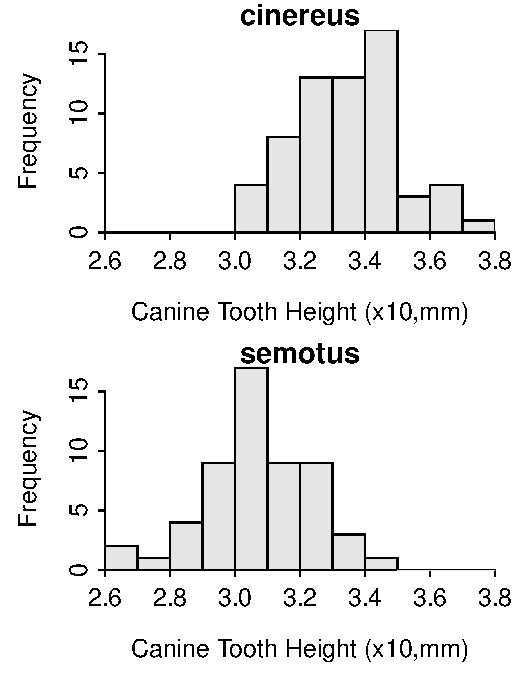
\includegraphics[width=.5\linewidth]{Figs/BatLogHist-1} 

}



\end{knitrout}
\newpage
\begin{knitrout}
\definecolor{shadecolor}{rgb}{0.969, 0.969, 0.969}\color{fgcolor}\begin{kframe}
\begin{alltt}
\hlstd{> }\hlkwd{histStack}\hlstd{(canine10}\hlopt{~}\hlstd{subsp,}\hlkwc{data}\hlstd{=bat,}\hlkwc{breaks}\hlstd{=}\hlkwd{seq}\hlstd{(}\hlnum{2.6}\hlstd{,}\hlnum{3.8}\hlstd{,}\hlnum{0.1}\hlstd{),}\hlkwc{xlim}\hlstd{=}\hlkwd{c}\hlstd{(}\hlnum{2.6}\hlstd{,}\hlnum{3.8}\hlstd{),}
\hlstd{ }          \hlkwc{col}\hlstd{=}\hlstr{"gray.colors"}\hlstd{,}\hlkwc{xlab}\hlstd{=xlbl,}\hlkwc{right}\hlstd{=}\hlnum{FALSE}\hlstd{)}
\end{alltt}
\end{kframe}

{\centering 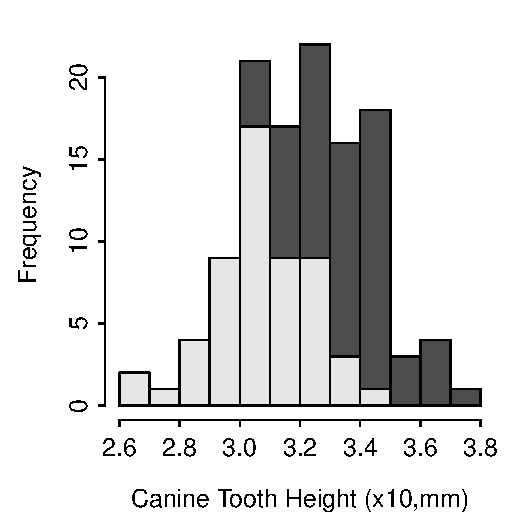
\includegraphics[width=.5\linewidth]{Figs/BatLogHist2-1} 

}



\end{knitrout}
\begin{knitrout}
\definecolor{shadecolor}{rgb}{0.969, 0.969, 0.969}\color{fgcolor}\begin{kframe}
\begin{alltt}
\hlstd{> }\hlkwd{plotBinResp}\hlstd{(subsp}\hlopt{~}\hlstd{canine10,}\hlkwc{data}\hlstd{=bat,}\hlkwc{breaks}\hlstd{=}\hlkwd{seq}\hlstd{(}\hlnum{2.6}\hlstd{,}\hlnum{3.8}\hlstd{,}\hlnum{0.1}\hlstd{),}\hlkwc{xlim}\hlstd{=}\hlkwd{c}\hlstd{(}\hlnum{2.6}\hlstd{,}\hlnum{3.8}\hlstd{),}
\hlstd{ }            \hlkwc{xlab}\hlstd{=xlbl,}\hlkwc{ylab}\hlstd{=ylbl)}
\end{alltt}
\end{kframe}

{\centering 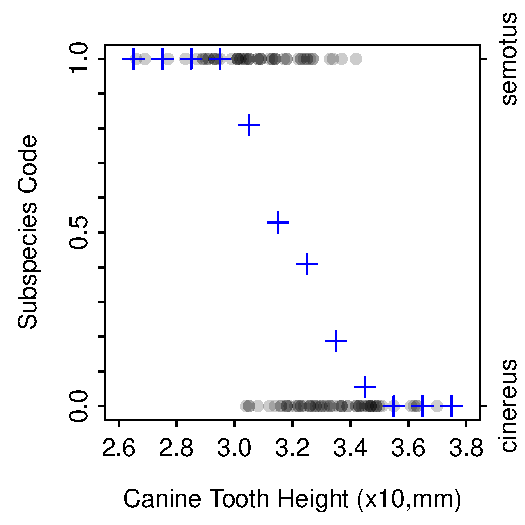
\includegraphics[width=.5\linewidth]{Figs/BatLogPlot-1} 

}



\end{knitrout}



\newpage
\subsection{Model Fitting and Examination}
\begin{knitrout}
\definecolor{shadecolor}{rgb}{0.969, 0.969, 0.969}\color{fgcolor}\begin{kframe}
\begin{alltt}
\hlstd{> }\hlstd{glm1} \hlkwb{<-} \hlkwd{glm}\hlstd{(subsp}\hlopt{~}\hlstd{canine10,}\hlkwc{data}\hlstd{=bat,}\hlkwc{family}\hlstd{=binomial)}
\hlstd{> }\hlkwd{fitPlot}\hlstd{(glm1,}\hlkwc{breaks}\hlstd{=}\hlkwd{seq}\hlstd{(}\hlnum{2.6}\hlstd{,}\hlnum{3.8}\hlstd{,}\hlnum{0.1}\hlstd{),}\hlkwc{xlab}\hlstd{=xlbl,}\hlkwc{ylab}\hlstd{=ylbl,}\hlkwc{main}\hlstd{=}\hlstr{""}\hlstd{)}
\end{alltt}
\end{kframe}

{\centering 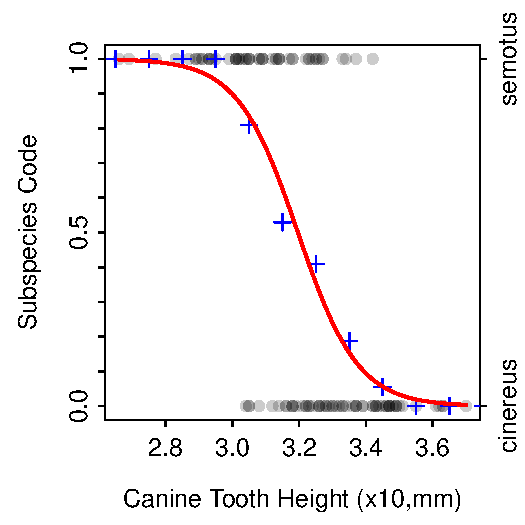
\includegraphics[width=.4\linewidth]{Figs/BatFLP-1} 

}


\begin{kframe}\begin{alltt}
\hlstd{> }\hlkwd{summary}\hlstd{(glm1)}
\end{alltt}
\begin{verbatim}

Coefficients:
            Estimate Std. Error z value Pr(>|z|)
(Intercept)   35.516      6.428   5.525 3.29e-08
canine10     -11.112      2.005  -5.543 2.97e-08

(Dispersion parameter for binomial family taken to be 1)

    Null deviance: 163.040  on 117  degrees of freedom
Residual deviance:  97.178  on 116  degrees of freedom
AIC: 101.18

Number of Fisher Scoring iterations: 5
\end{verbatim}
\begin{alltt}
\hlstd{> }\hlkwd{confint}\hlstd{(glm1)}
\end{alltt}


{\ttfamily\noindent\itshape\color{messagecolor}{Waiting for profiling to be done...}}\begin{verbatim}
                2.5 %   97.5 %
(Intercept)  24.21685 49.66132
canine10    -15.52430 -7.58941
\end{verbatim}
\end{kframe}
\end{knitrout}

\subsection{Interpretation of Slope}
\begin{knitrout}
\definecolor{shadecolor}{rgb}{0.969, 0.969, 0.969}\color{fgcolor}\begin{kframe}
\begin{alltt}
\hlstd{> }\hlstd{x1} \hlkwb{<-} \hlkwd{c}\hlstd{(}\hlnum{3}\hlstd{,}\hlnum{4}\hlstd{)}                  \hlcom{# purposely pick two canine10 values 1 unit apart}
\hlstd{> }\hlstd{( p1} \hlkwb{<-} \hlkwd{predict}\hlstd{(glm1,}\hlkwd{data.frame}\hlstd{(}\hlkwc{canine10}\hlstd{=x1)) )}
\end{alltt}
\begin{verbatim}
        1         2 
 2.179940 -8.931994 
\end{verbatim}
\begin{alltt}
\hlstd{> }\hlstd{p1[[}\hlnum{2}\hlstd{]]}\hlopt{-}\hlstd{p1[[}\hlnum{1}\hlstd{]]}
\end{alltt}
\begin{verbatim}
[1] -11.11193
\end{verbatim}
\begin{alltt}
\hlstd{> }\hlkwd{exp}\hlstd{(}\hlopt{-}\hlnum{11.112}\hlstd{)}                  \hlcom{# back-transformed 'slope' from summary() above}
\end{alltt}
\begin{verbatim}
[1] 1.493206e-05
\end{verbatim}
\begin{alltt}
\hlstd{> }\hlstd{( bp1} \hlkwb{<-} \hlkwd{exp}\hlstd{(p1) )}
\end{alltt}
\begin{verbatim}
           1            2 
8.8457728416 0.0001320944 
\end{verbatim}
\begin{alltt}
\hlstd{> }\hlstd{bp1[[}\hlnum{2}\hlstd{]]}\hlopt{/}\hlstd{bp1[[}\hlnum{1}\hlstd{]]}
\end{alltt}
\begin{verbatim}
[1] 1.493306e-05
\end{verbatim}
\end{kframe}
\end{knitrout}

\subsection{Predicting Probabilities}
\begin{knitrout}
\definecolor{shadecolor}{rgb}{0.969, 0.969, 0.969}\color{fgcolor}\begin{kframe}
\begin{alltt}
\hlstd{> }\hlstd{( p2} \hlkwb{<-} \hlkwd{predict}\hlstd{(glm1,}\hlkwd{data.frame}\hlstd{(}\hlkwc{canine10}\hlstd{=}\hlkwd{c}\hlstd{(}\hlnum{3}\hlstd{,}\hlnum{3.4}\hlstd{))) )}
\end{alltt}
\begin{verbatim}
        1         2 
 2.179940 -2.264834 
\end{verbatim}
\begin{alltt}
\hlstd{> }\hlkwd{exp}\hlstd{(p2)}\hlopt{/}\hlstd{(}\hlnum{1}\hlopt{+}\hlkwd{exp}\hlstd{(p2))}
\end{alltt}
\begin{verbatim}
         1          2 
0.89843357 0.09407761 
\end{verbatim}
\begin{alltt}
\hlstd{> }\hlkwd{predict}\hlstd{(glm1,}\hlkwd{data.frame}\hlstd{(}\hlkwc{canine10}\hlstd{=}\hlkwd{c}\hlstd{(}\hlnum{3}\hlstd{,}\hlnum{3.4}\hlstd{)),}\hlkwc{type}\hlstd{=}\hlstr{"response"}\hlstd{)}
\end{alltt}
\begin{verbatim}
         1          2 
0.89843357 0.09407761 
\end{verbatim}
\end{kframe}
\end{knitrout}

\subsection{X for a Certain Proportion}
\begin{knitrout}
\definecolor{shadecolor}{rgb}{0.969, 0.969, 0.969}\color{fgcolor}\begin{kframe}
\begin{alltt}
\hlstd{> }\hlstd{( cfs} \hlkwb{<-} \hlkwd{coef}\hlstd{(glm1) )}
\end{alltt}
\begin{verbatim}
(Intercept)    canine10 
   35.51574   -11.11193 
\end{verbatim}
\begin{alltt}
\hlstd{> }\hlstd{p} \hlkwb{<-} \hlnum{0.5}    \hlcom{# canine tooth height where subspecies ratio is 50/50}
\hlstd{> }\hlstd{( x} \hlkwb{<-} \hlstd{(}\hlkwd{log}\hlstd{(p}\hlopt{/}\hlstd{(}\hlnum{1}\hlopt{-}\hlstd{p))}\hlopt{-}\hlstd{cfs[[}\hlnum{1}\hlstd{]])}\hlopt{/}\hlstd{cfs[[}\hlnum{2}\hlstd{]] )}
\end{alltt}
\begin{verbatim}
[1] 3.19618
\end{verbatim}
\begin{alltt}
\hlstd{> }\hlkwd{predict}\hlstd{(glm1,}\hlkwd{data.frame}\hlstd{(}\hlkwc{canine10}\hlstd{=x),}\hlkwc{type}\hlstd{=}\hlstr{"response"}\hlstd{)}    \hlcom{# test the answer}
\end{alltt}
\begin{verbatim}
  1 
0.5 
\end{verbatim}
\begin{alltt}
\hlstd{> }\hlstd{p} \hlkwb{<-} \hlnum{0.9}    \hlcom{# length where 90% are semotus, 10% are cinereus}
\hlstd{> }\hlstd{(}\hlkwd{log}\hlstd{(p}\hlopt{/}\hlstd{(}\hlnum{1}\hlopt{-}\hlstd{p))}\hlopt{-}\hlstd{cfs[[}\hlnum{1}\hlstd{]])}\hlopt{/}\hlstd{cfs[[}\hlnum{2}\hlstd{]]}
\end{alltt}
\begin{verbatim}
[1] 2.998444
\end{verbatim}
\end{kframe}
\end{knitrout}

\newpage
\section{Bootstrapping}
\begin{knitrout}
\definecolor{shadecolor}{rgb}{0.969, 0.969, 0.969}\color{fgcolor}\begin{kframe}
\begin{alltt}
\hlstd{> }\hlstd{bc1} \hlkwb{<-} \hlkwd{bootCase}\hlstd{(glm1)}      \hlcom{# bootstrapping, be patient!}
\hlstd{> }\hlkwd{head}\hlstd{(bc1)}
\end{alltt}
\begin{verbatim}
     (Intercept)  canine10
[1,]    35.81998 -11.21662
[2,]    36.46938 -11.37874
[3,]    40.50277 -12.61516
[4,]    26.56209  -8.20114
[5,]    40.00093 -12.50260
[6,]    35.67100 -11.02964
\end{verbatim}
\begin{alltt}
\hlstd{> }\hlkwd{confint}\hlstd{(bc1)}
\end{alltt}
\begin{verbatim}
              95% LCI  95% UCI
(Intercept)  26.24424 50.73736
canine10    -15.88791 -8.20068
\end{verbatim}
\begin{alltt}
\hlstd{> }\hlstd{predProb} \hlkwb{<-} \hlkwa{function}\hlstd{(}\hlkwc{x}\hlstd{,}\hlkwc{alpha}\hlstd{,}\hlkwc{beta1}\hlstd{)} \hlkwd{exp}\hlstd{(alpha}\hlopt{+}\hlstd{beta1}\hlopt{*}\hlstd{x)}\hlopt{/}\hlstd{(}\hlnum{1}\hlopt{+}\hlkwd{exp}\hlstd{(alpha}\hlopt{+}\hlstd{beta1}\hlopt{*}\hlstd{x))}
\hlstd{> }\hlkwd{predProb}\hlstd{(}\hlnum{3}\hlstd{,}\hlkwd{coef}\hlstd{(glm1)[[}\hlnum{1}\hlstd{]],}\hlkwd{coef}\hlstd{(glm1)[[}\hlnum{2}\hlstd{]])}
\end{alltt}
\begin{verbatim}
[1] 0.8984336
\end{verbatim}
\begin{alltt}
\hlstd{> }\hlstd{p3} \hlkwb{<-} \hlkwd{predProb}\hlstd{(}\hlnum{3}\hlstd{,bc1[,}\hlnum{1}\hlstd{],bc1[,}\hlnum{2}\hlstd{])}
\hlstd{> }\hlkwd{head}\hlstd{(p3)}
\end{alltt}
\begin{verbatim}
[1] 0.8975332 0.9115875 0.9344588 0.8763892 0.9236589 0.9296982
\end{verbatim}
\begin{alltt}
\hlstd{> }\hlkwd{quantile}\hlstd{(p3,}\hlkwd{c}\hlstd{(}\hlnum{0.025}\hlstd{,}\hlnum{0.975}\hlstd{))}
\end{alltt}
\begin{verbatim}
     2.5%     97.5% 
0.8118832 0.9636279 
\end{verbatim}
\begin{alltt}
\hlstd{> }\hlstd{predX} \hlkwb{<-} \hlkwa{function}\hlstd{(}\hlkwc{p}\hlstd{,}\hlkwc{alpha}\hlstd{,}\hlkwc{beta1}\hlstd{) (}\hlkwd{log}\hlstd{(p}\hlopt{/}\hlstd{(}\hlnum{1}\hlopt{-}\hlstd{p))}\hlopt{-}\hlstd{alpha)}\hlopt{/}\hlstd{beta1}
\hlstd{> }\hlstd{x50} \hlkwb{<-} \hlkwd{predX}\hlstd{(}\hlnum{0.5}\hlstd{,bc1[,}\hlnum{1}\hlstd{],bc1[,}\hlnum{2}\hlstd{])}
\hlstd{> }\hlkwd{head}\hlstd{(x50)}
\end{alltt}
\begin{verbatim}
[1] 3.193473 3.205047 3.210642 3.238829 3.199409 3.234102
\end{verbatim}
\begin{alltt}
\hlstd{> }\hlkwd{quantile}\hlstd{(x50,}\hlkwd{c}\hlstd{(}\hlnum{0.025}\hlstd{,}\hlnum{0.975}\hlstd{))}
\end{alltt}
\begin{verbatim}
    2.5%    97.5% 
3.149542 3.241326 
\end{verbatim}
\end{kframe}
\end{knitrout}


\newpage
\section{Solar Panel Offer Data}
\begin{knitrout}
\definecolor{shadecolor}{rgb}{0.969, 0.969, 0.969}\color{fgcolor}\begin{kframe}
\begin{alltt}
\hlstd{> }\hlstd{sp} \hlkwb{<-} \hlkwd{read.csv}\hlstd{(}\hlstr{"https://raw.githubusercontent.com/droglenc/NCData/master/SolarOffer.csv"}\hlstd{)}
\hlstd{> }\hlkwd{str}\hlstd{(sp)}
\end{alltt}
\begin{verbatim}
'data.frame':	30 obs. of  5 variables:
 $ income   : int  80 60 35 45 29 43 34 104 102 59 ...
 $ age      : int  30 34 25 27 23 28 24 43 46 36 ...
 $ takeoffer: Factor w/ 2 levels "decline","take": 2 2 1 1 1 1 1 2 2 1 ...
 $ mortgage : int  2000 2100 1500 1800 1900 1600 1500 2400 2700 2600 ...
 $ famsize  : int  4 3 2 4 2 3 1 5 3 2 ...
\end{verbatim}
\begin{alltt}
\hlstd{> }\hlstd{xlbl} \hlkwb{<-} \hlstr{"Family Income (1000s)"}
\hlstd{> }\hlstd{ylbl} \hlkwb{<-} \hlstr{"Response to Offer"}
\end{alltt}
\end{kframe}
\end{knitrout}

\begin{knitrout}
\definecolor{shadecolor}{rgb}{0.969, 0.969, 0.969}\color{fgcolor}\begin{kframe}
\begin{alltt}
\hlstd{> }\hlkwd{plotBinResp}\hlstd{(takeoffer}\hlopt{~}\hlstd{income,}\hlkwc{data}\hlstd{=sp,}\hlkwc{xlab}\hlstd{=xlbl,}\hlkwc{ylab}\hlstd{=ylbl,}\hlkwc{breaks}\hlstd{=}\hlkwd{seq}\hlstd{(}\hlnum{25}\hlstd{,}\hlnum{135}\hlstd{,}\hlnum{5}\hlstd{))}
\end{alltt}
\end{kframe}

{\centering 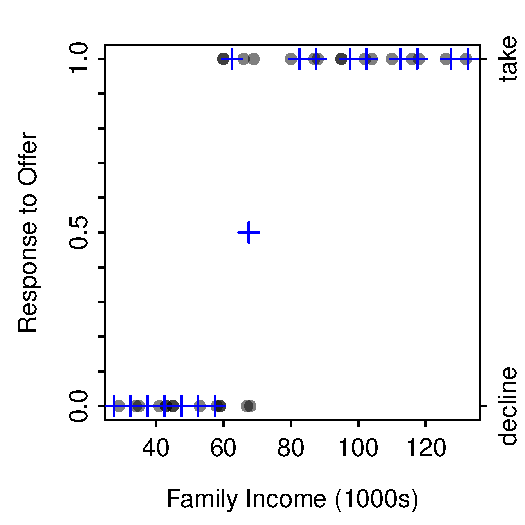
\includegraphics[width=.4\linewidth]{Figs/SolarLogPlot-1} 

}


\begin{kframe}\begin{alltt}
\hlstd{> }\hlstd{glm2} \hlkwb{<-} \hlkwd{glm}\hlstd{(takeoffer}\hlopt{~}\hlstd{income,}\hlkwc{data}\hlstd{=sp,}\hlkwc{family}\hlstd{=binomial)}
\hlstd{> }\hlkwd{summary}\hlstd{(glm2)}
\end{alltt}
\begin{verbatim}

Coefficients:
             Estimate Std. Error z value Pr(>|z|)
(Intercept) -12.84503    6.16398  -2.084   0.0372
income        0.19934    0.09774   2.039   0.0414

(Dispersion parameter for binomial family taken to be 1)

    Null deviance: 41.455  on 29  degrees of freedom
Residual deviance: 13.035  on 28  degrees of freedom
AIC: 17.035

Number of Fisher Scoring iterations: 8
\end{verbatim}
\begin{alltt}
\hlstd{> }\hlkwd{fitPlot}\hlstd{(glm2,}\hlkwc{xlab}\hlstd{=xlbl,}\hlkwc{ylab}\hlstd{=ylbl,}\hlkwc{breaks}\hlstd{=}\hlkwd{seq}\hlstd{(}\hlnum{25}\hlstd{,}\hlnum{135}\hlstd{,}\hlnum{5}\hlstd{),}\hlkwc{main}\hlstd{=}\hlstr{""}\hlstd{)}
\end{alltt}
\end{kframe}

{\centering 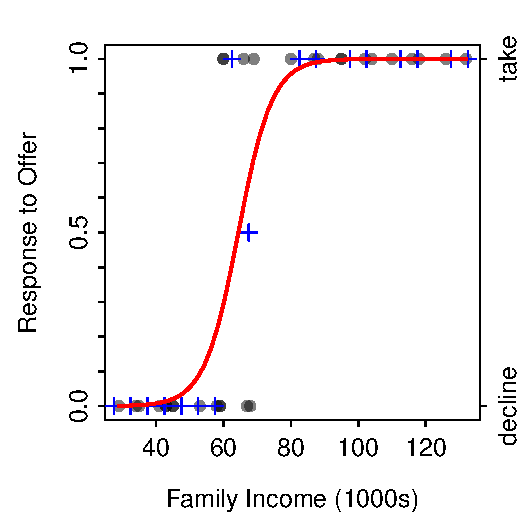
\includegraphics[width=.4\linewidth]{Figs/SolarLogPlot-2} 

}


\begin{kframe}\begin{alltt}
\hlstd{> }\hlstd{p} \hlkwb{<-} \hlnum{0.25}
\hlstd{> }\hlstd{(}\hlkwd{log}\hlstd{(p}\hlopt{/}\hlstd{(}\hlnum{1}\hlopt{-}\hlstd{p))}\hlopt{-}\hlkwd{coef}\hlstd{(glm2)[}\hlnum{1}\hlstd{])}\hlopt{/}\hlkwd{coef}\hlstd{(glm2)[}\hlnum{2}\hlstd{]}
\end{alltt}
\begin{verbatim}
(Intercept) 
   58.92646 
\end{verbatim}
\begin{alltt}
\hlstd{> }\hlkwd{predict}\hlstd{(glm2,}\hlkwd{data.frame}\hlstd{(}\hlkwc{income}\hlstd{=}\hlnum{80}\hlstd{),}\hlkwc{type}\hlstd{=}\hlstr{"response"}\hlstd{)}
\end{alltt}
\begin{verbatim}
        1 
0.9569831 
\end{verbatim}
\end{kframe}
\end{knitrout}

\end{document}
